\documentclass[twoside,leqno,twocolumn]{article}

\usepackage{ltexpprt}
\usepackage{amsmath}
\usepackage{graphicx,psfrag,epsf,subcaption}
\usepackage{enumerate}
\usepackage{natbib}
\usepackage[export]{adjustbox}

%\def\footnoterule{\hrule \kern \dimexpr#1}
\begin{document}

\title{Matrix Explorer: A Web Application for Data Exploration%
	\thanks{{This work is graciously supported by the Defense Advanced Research Projects Agency (DARPA) SIMPLEX program through SPAWAR contract N66001-15-C-4041 and DARPA GRAPHS N66001-14-1-4028}}
}


\author{Ivan A. Kuznetsov%
	\thanks{Department of Biomedical Engineering,  The Johns Hopkins University, Baltimore, Maryland 21218, USA}%
	\and
	Joshua T. Vogelstein%
	\footnotemark[2]
	\thanks{Institute for Computational Medicine, Center for Imaging Science, The Johns Hopkins University, Baltimore, Maryland 21218, USA}
}
\date{}
\maketitle

\begin{abstract}\small\baselineskip=9pt
Exploration and visualization of data is crucial to driving discovery across a multitude of different basic science fields. Unfortunately, given the vast array of various statistical tools that have been developed, finding the proper techniques to explore a novel dataset is more of an art than an exact science. Hence, researchers often spend unnecessary time choosing tools to explore their data, and worse, sometimes choose tools with known numerical issues.  In this paper we describe Matrix Explorer, a novel data exploration and visualization Web application. The tool allows users to upload and analyze matrix valued datasets. Within Matrix Explorer we have incorporated reference techniques for any sort of data analyses, such as data visualization via heatmaps, scatter/line plots, marginal distributions, and two-dimensional embedding and data exploration via k-means clustering, dendrograms, correlation matrix computation, and outlier detection. We validated Matrix Explorer by showing that it produces reasonable results for the iris flower dataset. We then used Matrix Explorer to analyze a novel SPECT brain imaging dataset. We determined for the first time that SPECT could be used for single subject classification of sex, suggesting that it might be a viable low-cost method for brain imaging assays, unlike magnetic resonance imaging.
\end{abstract}



\section{Introduction}
\label{sec:intro}

John Tukey originally formalized exploratory data analysis through his work in the mid-twentieth century \cite{tukey1962future}. Although he is perhaps most well known for highlighting the importance of proper analysis, Tukey's brilliance also stemmed from his careful, pragmatic decisions about what sort of analysis to do. This latter fact is even more important now, half a century later, as statisticians possess a near infinite number of tools to facilitate data analysis, and it is increasingly difficult to choose the optimal subset of techniques to solve a given problem. As a result, exploratory analysis of novel datasets remains more of an art than an exact science. The result of this phenomenon is that a large quantity of collected data, especially in the basic sciences, is either poorly or inefficiently analyzed, likely decreasing the pace of new discoveries and increasing the chances of failed reproductions. This overflow of knowledge is not unique to exploratory data analysis. Other fields, most notably clinical medicine, have dealt with this issue by adopting standards of care, often driven by simple checklists. 

In light of these facts, we propose a checklist for exploratory data analysis using modern tools. Simultaneously, to maximize efficiency, we develop a code base to simplify these analyses to the point that they can be done without ever writing a line of code. To the best to of our knowledge, such a tool does not yet exist. The R, MATLAB, and Python languages and associated toolboxes and packages still require users to write significant code for even the simplest analysis. Other attempts at making data analysis more efficient, such as GGobi and ViSta, as described in \cite{swayne2003ggobi} and \cite{valero2011using} respectively, have not resolved the issue, requiring a significant learning curve to utilize. There have been several recent commerical attempts to address this issue. For example, Ayasdi provides a very nice interface, although it uses custom algorithms that are not open source. Tableau is another popular option that requires a contract and is not open source. 

In this paper we describe Matrix Explorer (MX), our first attempt at developing such a system. MX is a novel data exploration web application built via the R Shiny package. Within MX we have included the techniques which we deem best practice whenever starting a new exploratory analysis task. MX provides users with any level of knowledge of statistics the tools necessary to conduct a basic characterization of their data.

\section{Methods \& Result Validation}
\label{sec:meth}

MX is implemented via the R Shiny package, which allows for the construction of interactive web applications which use R as their backend. The Shiny server is hosted on a Docker instance. The functionality of MX is divided into several different submodules, organized as tabs in the web application, which we  describe in depth below. Furthermore, we provide visualizations and validation of the ability of MX to allow for basic data analysis by provided by exploring the iris flower dataset. 

The iris dataset is composed of 50 samples from each of three species of iris flower (\textit{setosa}, \textit{virginica}, and \textit{versicolor}). For each sample four features are measured, specifically the length and width of the sepal and petals. For the purposes of the validation, we added a fifth feature column which gives the class label of each sample. We now seek to show that MX can detect that the samples should cluster into three distinct groups.

\subsection{Data Upload \& Selection}
\label{subsec:SubSecUpload}

Upon opening the application, the user is first prompted to upload a dataset. Note that MX assumes that rows in the dataset represent samples and columns represent features. Once uploading is complete, the user may then select the rows and columns that he or she wishes to analyze and also flag a specific column as a class label column. The current implementation accepts comma separated variable (CSV) files and is optimized for sizes below 1 gigabyte. Hence, we converted our iris dataset to CSV format and uploaded it to MX using the interface.

\subsection{Heatmap \& Dendrogram}
\label{subsec:SubSecHeatmap}

\begin{figure}[t!]
	\centering
	\begin{subfigure}[t]{0.46\textwidth}
		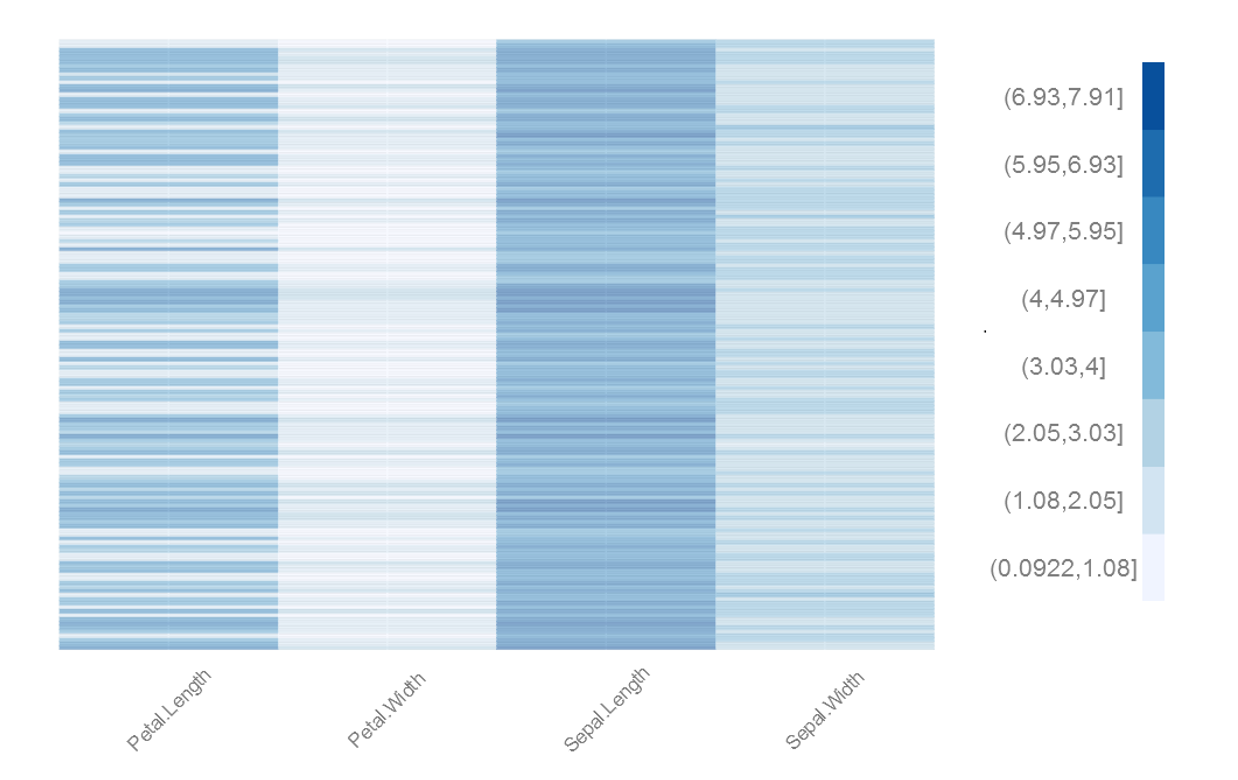
\includegraphics[width=\textwidth,valign=t]{Figures/Iris/HeatmapRawnodendro.png}
		\subcaption{}
		\label{fig:FigHeatmapRawnodendro}
	\end{subfigure}
	\begin{subfigure}[t]{0.46\textwidth}
		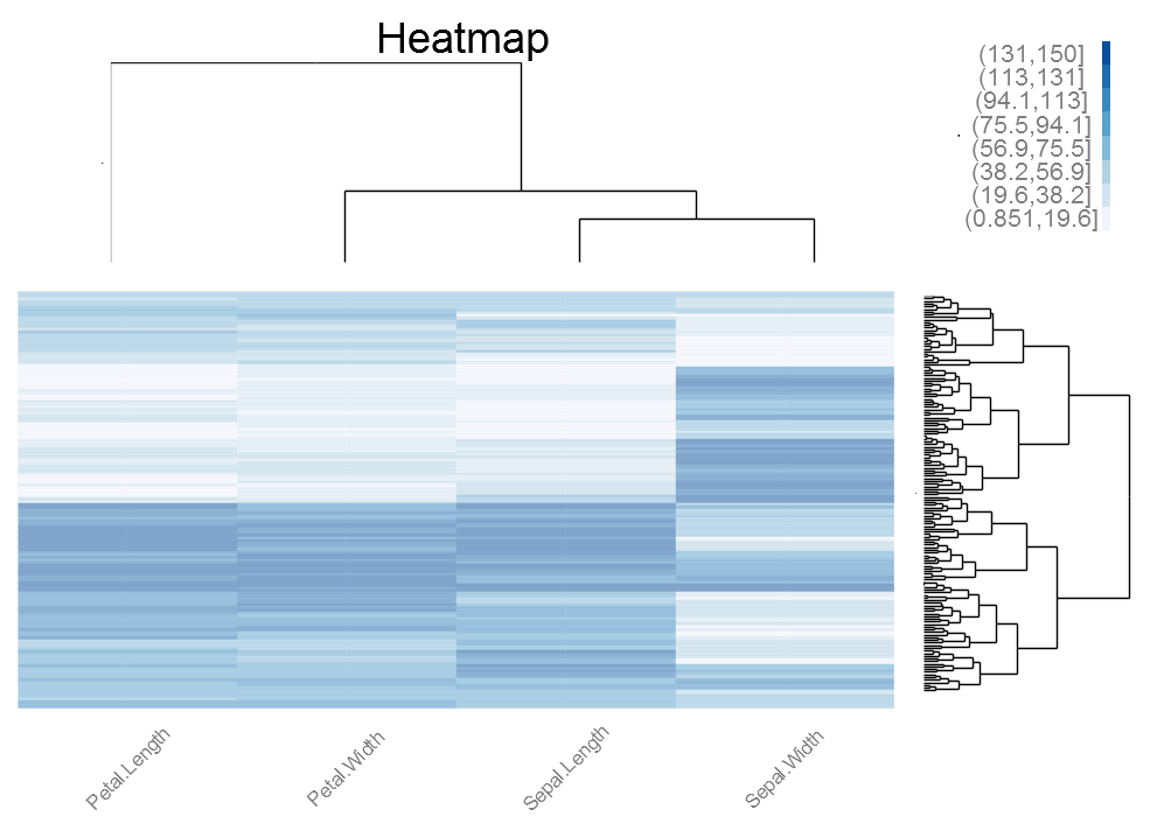
\includegraphics[width=\textwidth,valign=t]{Figures/Iris/HeatmapRanksDendro.png}
		\subcaption{}
		\label{fig:FigHeatmapRanksdendro}
	\end{subfigure}
	%\vspace{-3\baselineskip}
	\caption{Heatmap of iris dataset for various visualization options. Sample labels are not shown. (a) Heatmap of raw data. Note that there is no evidence for the existence of clusters. (b) Heatmap of data converted to rank with dendrogram and associated row and column sorting. The existence of at least two clusters is clear.}
	\label{fig:FigHeatmap}
\end{figure}

A heatmap provides the most direct way of visualizing the data, besides simply looking at it as a data table. Clear trends in the data are often obscured on a heatmap because of varying ranges amongst features. Different normalization schemes can resolve this issue. The usefulness of heatmaps is further increased by the ability to be displayed alongside dendrograms, which allows for easy sorting and clustering.

MX allows users to construct a heatmap of their data and gives them the option to normalize it via conversion to z-scores, quantiles, or ranks. Furthermore, for datasets with less than 100 rows and columns, MX uses hierarchical clustering to compute a dendrogram of the dataset and display it, reordering the columns and rows as necessary. 

We used this feature of MX to do our initial exploration of the iris dataset. Note that a simple heatmap of the unnormalized dataset, as shown in Figure~\ref{fig:FigHeatmapRawnodendro}, is not particularly useful. There is no clear structure to the data. This is where normalization schemes as well as dendrograms and the associated sorting they impose upon the rows and columns of the heatmap become useful. A heatmap and dendrogram for the ranked data is shown in Figure~\ref{fig:FigHeatmapRanksdendro}. Note that the existence of at least 2 clusters is now apparent.

\subsection{Sample Summary}
\label{subsec:SubSecSample}

\begin{figure}[t!]
	\centering
	\begin{subfigure}[t]{0.48\textwidth}
		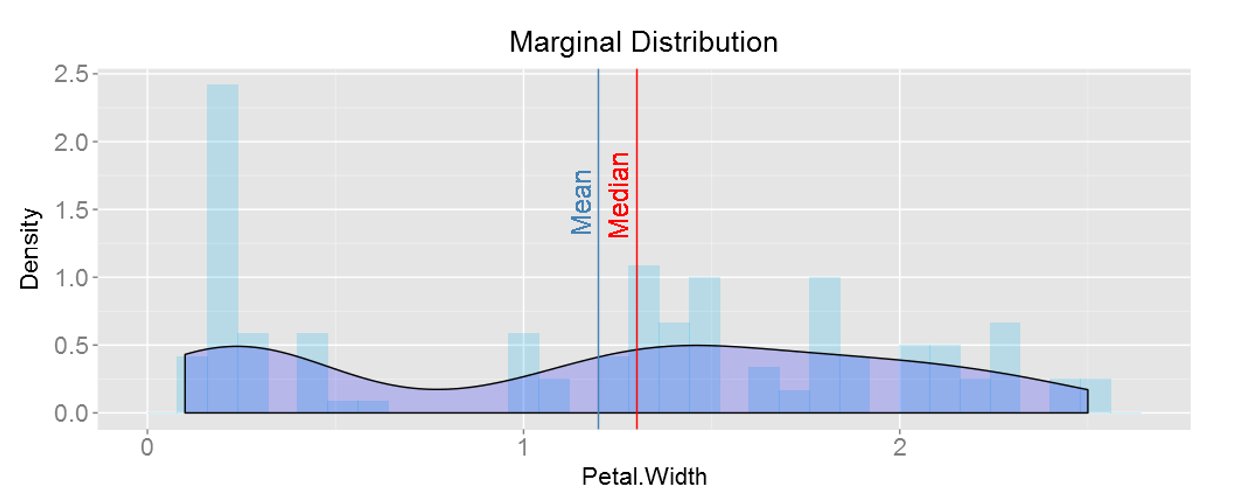
\includegraphics[width=\textwidth,valign=t]{Figures/Iris/MarginalPetalWidthnocond.png}
		\subcaption{}
		\label{fig:FigMarginalNoCond}
	\end{subfigure}
	\begin{subfigure}[t]{0.48\textwidth}
		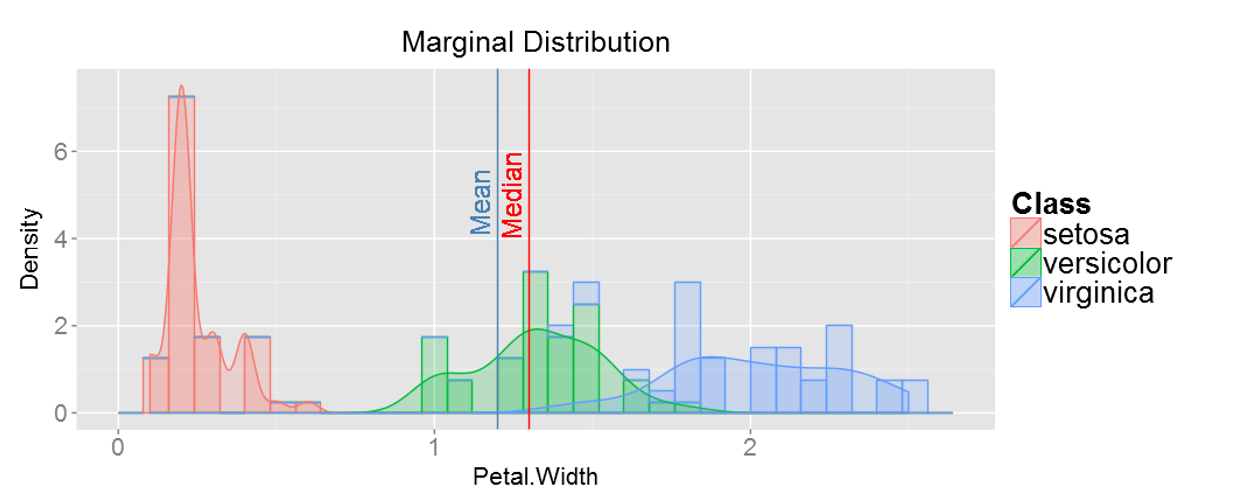
\includegraphics[width=\textwidth,valign=t]{Figures/Iris/MarginalPetalWidth.png}
		\subcaption{}
		\label{fig:FigMarginal}
	\end{subfigure}
	%\vspace{-3\baselineskip}
	\caption{Marginal of the petal width feature of the iris dataset. (a) Histogram and kernel density estimate of the samples without conditioning on class. Note that it is unclear whether the distribution is multi-modal. (b) Histogram and kernel density estimate of the samples after conditioning on class. It is now clear that the marginal distribution is tri-modal.}
	\label{fig:FigSample}
\end{figure}

One of the initial steps in exploring a new dataset is to look at the marginal distributions of the individual feature columns, as this helps direct future work. MX allows users to visualize these marginal distributions. MX can generate either a histogram, a kernel density estimate, or a overlay of both. The mean and median is indicated on the plot. Additionally, if the user labeled a feature as a class label column, he or she has the option of conditioning the marginal on classes. This latter feature is incredibly useful for feature selection and determining the separability of the data based on class label within the feature space.

We used MX to construct the feature marginals. The distribution for petal width is shown in Figure~\ref{fig:FigMarginalNoCond}. Note that it is unclear whether the distribution is multi-modal and if it is, out of how many modes compose it. It is also not clear how useful this feature is for separating the samples into the different iris classes. This is where conditioning on classes, shown in Figure~\ref{fig:FigMarginal}, becomes useful. It is now clear that the marginal is essentially tri-modal and that the petal width feature does a good job of separating the samples into the three classes.

\subsection{Outliers}
\label{subsec:SubSecOutliers}

\begin{figure}[t!]
	\centering
	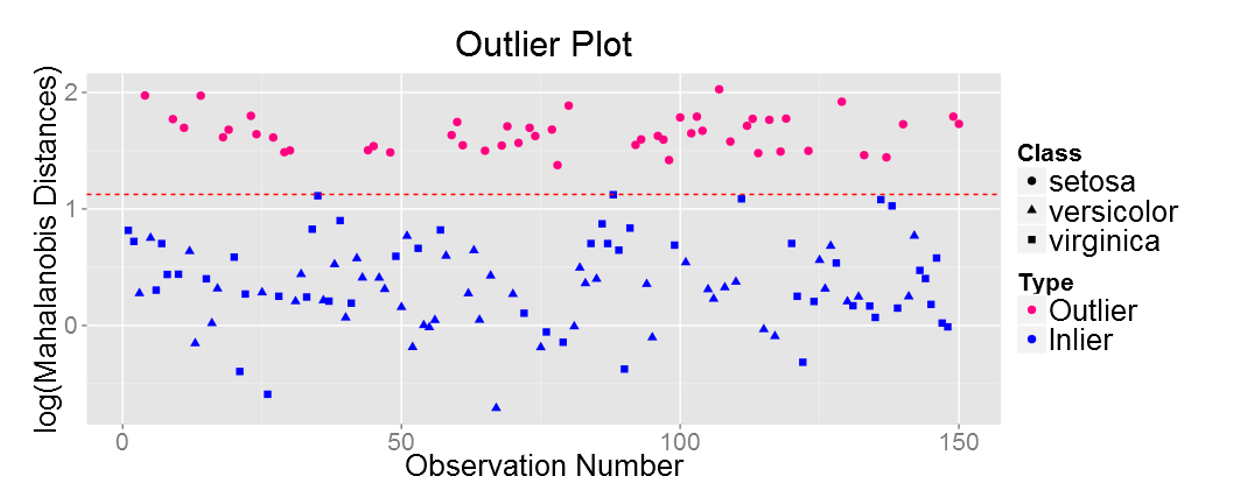
\includegraphics[width=0.48\textwidth]{Figures/Iris/OutliersIris.png}
	\caption{Robust Mahalanobis distances with choice of alpha cut-off value to reject samples as outliers on the iris dataset. Note that 51 of the 150 samples are flagged as outliers. Such as large number of outliers usually indicates the existence of samples which belong to a separate group than the rest of the data. As a matter of fact, 50 of these 51 samples belong to the \textit{Iris setosa} class, which is apparently quite far from the samples which belong to the \textit{Iris virginica} and \textit{Iris versicolor} classes.}
	\label{fig:FigOutliers}
\end{figure}

Outlier detection is often an important step in the data analytic process. In order to determine outliers it is necessary to first establish a distance metric to determine how far away a specific sample is from other samples. In this case, robust Mahalanobis distances were used, as described in \cite{hubert2008high}. Briefly, a robust estimate of the sample mean and covariance was first approximated via either: 1) the fast minimum covariance determinant algorithm (FAST-MCD) as described in \cite{rousseeuw1999fast} or 2) the Orthogonalized Gnanadesikan-Kettenring algorithm (OGK) as described in \cite{maronna2002robust}. Specifically, FAST-MCD was used for low dimensional datasets, while OGK was used for high dimensional datasets due to the fact that FAST-MCD scales poorly with increasing dimensionality. Next, using these robust measures, the Mahalanobis distance of each sample was computed. As explained by \cite{hardin2012distribution}, the squares of the robust Mahalanobis distances are approximately distributed $\chi^2_n$, where $n$ is the dimensionality of the dataset. It is then possible to define an alpha value above which to reject a sample as an outlier. 

MX allows the user to set this alpha value and graphically displays the robust Mahalnobis distances and resulting threshold. The robust Mahalanobis distances for the iris data are shown in Figure~\ref{fig:FigOutliers}. MX labels 51 of the 150 samples as outliers, which is a very high fraction. It is quite unlikely that all of these are actually outliers, and it is more likely that the samples which were flagged as outliers actually mostly belong to a single class of iris flower that is simply far from the other two classes. If we examine the class labels (indicated by symbol), this is exactly what we find: 50 of these 51 samples belong to the \textit{Iris setosa} class, which is apparently  far from the samples which belong to the \textit{Iris virginica} and \textit{Iris versicolor} classes. Interestingly, the outlier analysis does not indicate a difference in distance between the samples from the \textit{Iris virginica} and \textit{Iris versicolor} class. 

\subsection{Correlation}
\label{subsec:SubSecCorrelation}

Knowledge of which features are correlated is highly relevant for both assumption checking and feature selection purposes. Similarly, correlations may aid in providing an intuitive understanding of the underlying patterns within the data. For example, in gene expression datasets these correlations may suggest the biological importance of various genetic markers. To see an example of when this is useful, we refer the reader to \cite{shi2012unsupervised}.

MX computes the Pearson's correlation amongst features and displays it to the user. To better understand the interactions and distributions of features, MX can also compute the Euclidean distance between features. To account for scaling effects, users have the option of pre-processing the data via conversion to z-scores, quantiles, or ranks. Furthermore, users can remove the outliers detected in the outlier tab from the data before computing the metrics. Using these features on the iris data, we found that all 4 of the features are strongly correlated with one another (data not shown).

\subsection{Feature Summary}
\label{subsec:SubSecFeature}

\begin{figure}[t!]
	\centering
	\begin{subfigure}[t]{0.48\textwidth}
		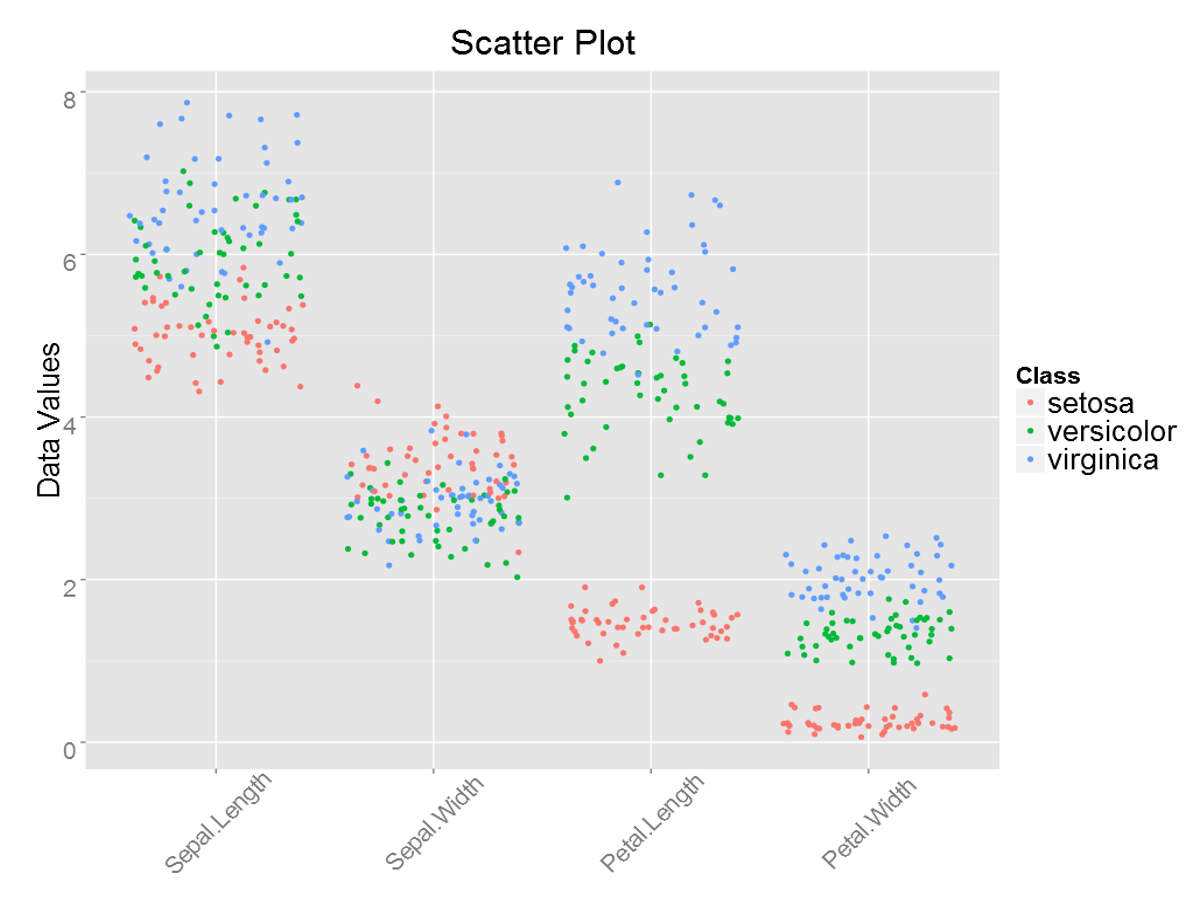
\includegraphics[width=\textwidth,valign=t]{Figures/Iris/ScatterColor.png}
		\subcaption{}
		\label{fig:FigScatter}
	\end{subfigure}
	\begin{subfigure}[t]{0.48\textwidth}
		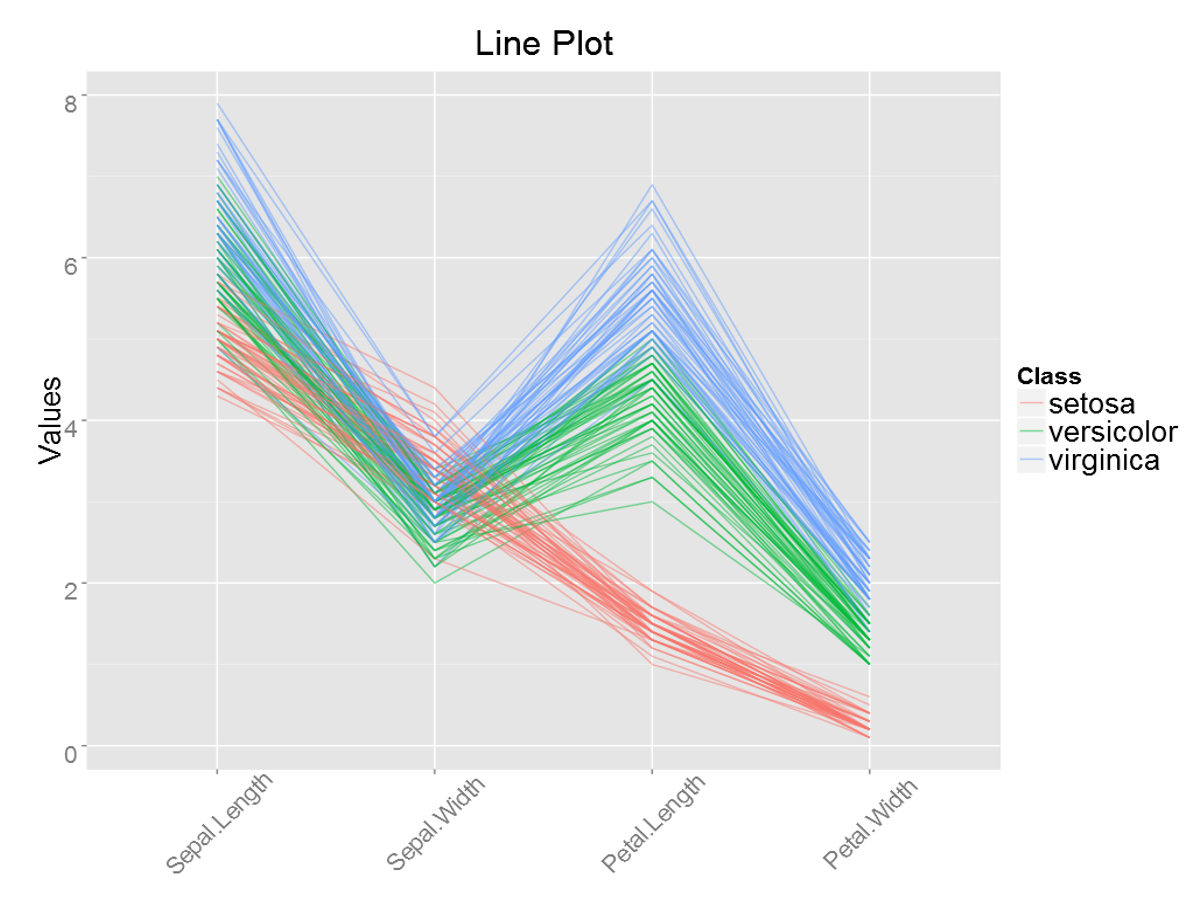
\includegraphics[width=\textwidth,valign=t]{Figures/Iris/LineColor.png}
		\subcaption{}
		\label{fig:FigLine}
	\end{subfigure}
	%\vspace{-3\baselineskip}
	\caption{Visualization of the samples across all the features in the iris dataset. (a) Jittered scatter plot of the sample values across the features and colored based on class label. Note that the multi-modal nature of the petal width and petal length marginal distributions is clear. It is also apparent that the samples from the \textit{Iris setosa} class are very different from the samples from the other two classes. (b) Line plot showing the behavior of individual samples across the features. Visually, it is clear how differently the samples from the \textit{Iris setosa} class behave compared to samples from the other classes. Note also that we can now visually see the absence of actual outliers.}
	\label{fig:FigFeature}
\end{figure}

MX allows users to visualize the marginal distributions of all the features on the same plot. MX provides a number of different display options for this: a jittered scatter plot, a line plot (where each line represents the values a sample takes on at the corresponding feature), a vector of sample means with standard error bars, a box plot, and a violin plot. To ensure that outliers do not skew the visualizations, users have the options of removing outliers detected in the outlier tab from the dataset before generating the plots. 

A jittered scatter plot of the iris data, colored by class label, is shown in Figure~\ref{fig:FigScatter}. The multi-modal nature of the petal length and width features is clear from the plot. Furthermore, the two petal related features seem to be optimal for separating the data into the three classes. Just like from the outlier analysis, it is apparent here that the samples from the \textit{Iris setosa} class differ strongly from the samples from the \textit{Iris virginica} and \textit{Iris versicolor} classes. A line plot colored by class label of the same data is shown in Figure~\ref{fig:FigLine}. Again, we see how similar the samples from the \textit{Iris virginica} and \textit{Iris versicolor} classes are to each other and how different they are from the samples from the \textit{Iris setosa} class. Interestingly, we can now visually see that there are no obvious outliers in the data. These observations give credence to our statement in the previous section that the samples flagged as outliers by MX were not ``real" outliers, but actually were just samples from a single class.

\subsection{Embedding \& Clustering}
\label{subsec:SubSecEmbedding}

\begin{figure}[t]
	\centering
	\begin{subfigure}[t]{0.48\textwidth}
		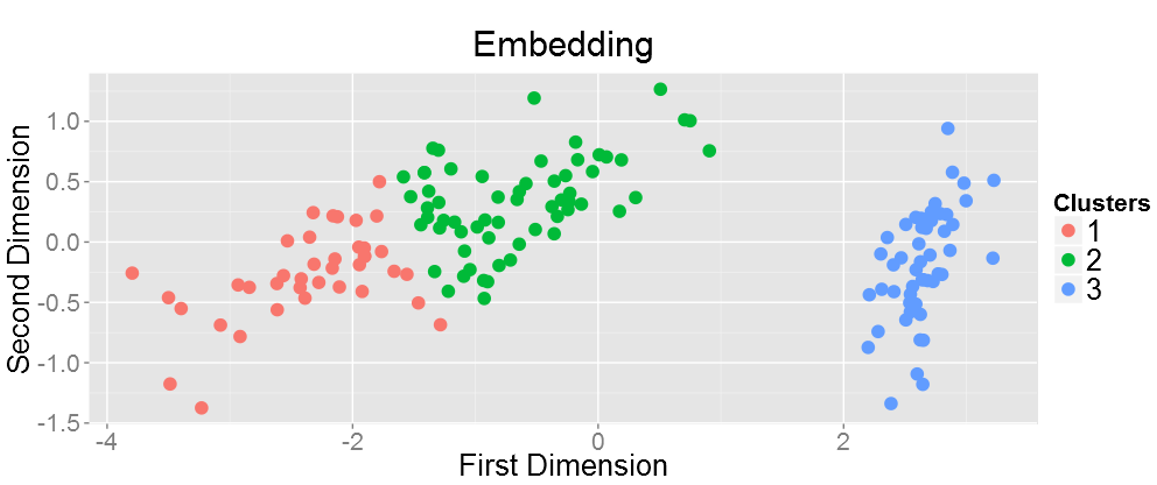
\includegraphics[width=\textwidth,valign=t]{Figures/Iris/EmbedRaw.png}
		\subcaption{}
		\label{fig:FigEmbedRaw}
	\end{subfigure}
	\begin{subfigure}[t]{0.48\textwidth}
		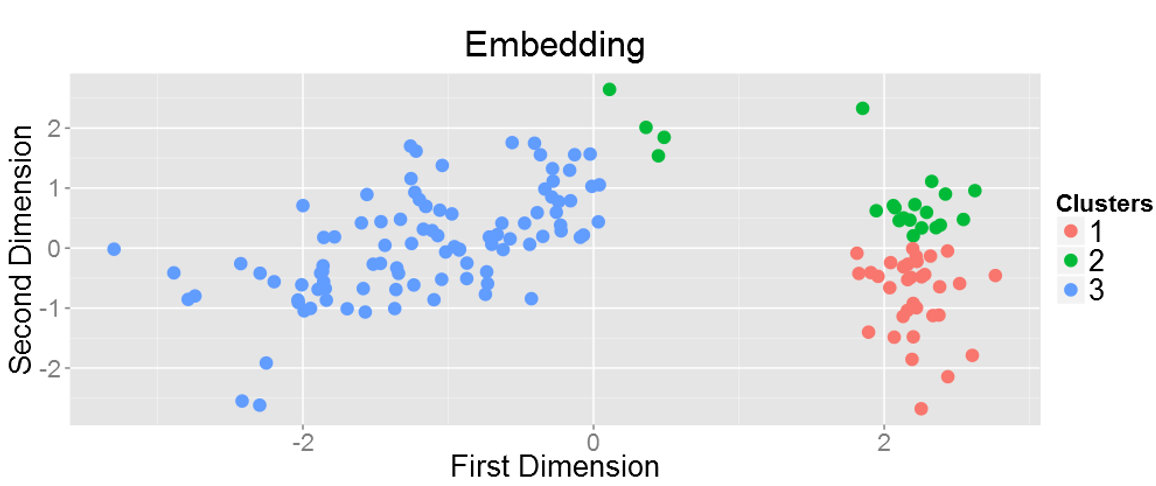
\includegraphics[width=\textwidth,valign=t]{Figures/Iris/EmbedZ.png}
		\subcaption{}
		\label{fig:FigEmbedZ}
	\end{subfigure}
	%\vspace{-3\baselineskip}
	\caption{Two-dimensional embedding of samples using PCA followed by coloring using labels given by k-means clustering with \textit{k = 3} using (a) raw data and (b) z-score normalized data. Note that the k-means result is significantly worse in (b) compared to (a), to the point that it obfuscates the obvious existence of clear clusters.}
	\label{fig:FigEmbedding}
\end{figure}

One of the most intuitive ways of visualizing bivariate data is a scatter plot. Although this is not directly possible for data with more than two dimensions, various dimensionality reduction techniques can be used to embed the data within a two-dimensional coordinate system for simple examination of general structure and clustering. Dimensionality reduction techniques can be further reduced into linear and non-linear methods, both of which have their own unique advantages and disadvantages. For an overview of techniques we refer the reader to \cite{van2009dimensionality}. Within MX we have implemented one linear method, principle component analysis (PCA), and one non-linear method, t-distributed stochastic neighbor embedding (tSNE) \cite{van2008visualizing}.

Note that PCA is extremely sensitive to (1) the scaling of the data and to the (2) presence of outliers.  Hence, to overcome (1), MX allows users to normalize the feature columns by converting either to z-scores, quantiles, or ranks. Note that conversion to quantiles or ranks also decreases the sensitivity of the embedding to outliers, hence aiding in overcoming (2). MX also allows users to resolve (2) more directly by giving them the option to remove the outliers detected in the outliers tab before generating the visualization. To inform the users of how much variance was lost by embedding the data set into two dimensions, MX also displays a scree plot, which indicates the percentage of retained variance after PCA. 

Two-dimensional embedding via PCA for the raw  and z-score normalized iris data after coloring using labels attained via k-means with \textit{k = 3} is shown in Figure~\ref{fig:FigEmbedRaw} and Figure~\ref{fig:FigEmbedZ}, respectively. Note that the k-means clustering result for the z-score normalized data is far worse than the result for the raw data, as it does not indicate the existence of two easily separable clusters. This suggests that the current standard of normalizing to z-scores is not optimal in this setting. As we have seen above, the cluster that lies far away from the other two is likely composed of samples which belong to the \textit{Iris setosa} class.

\section{Analysis of a Novel SPECT Dataset}

\begin{figure}[t]
	\centering
	\begin{subfigure}[t]{0.48\textwidth}
		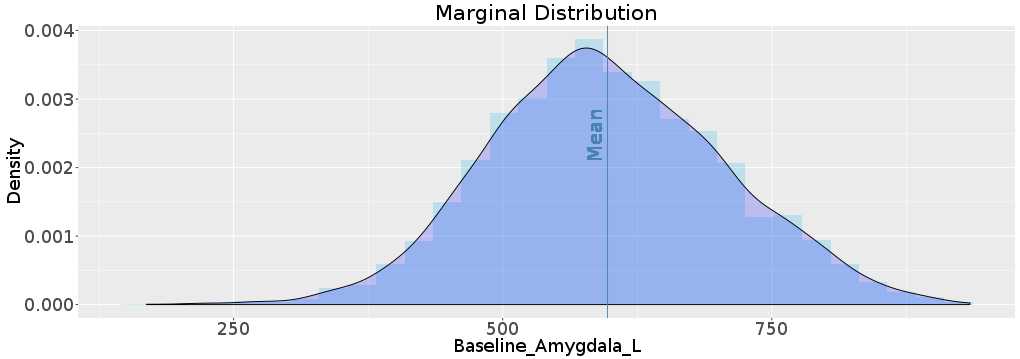
\includegraphics[width=\textwidth,valign=t]{Figures/Spect_Gender/NonClass_Baseline_Amygdala_L.png}
		\subcaption{}
		\label{fig:FigSpecNoClassMarginal}
	\end{subfigure}
	\begin{subfigure}[t]{0.48\textwidth}
		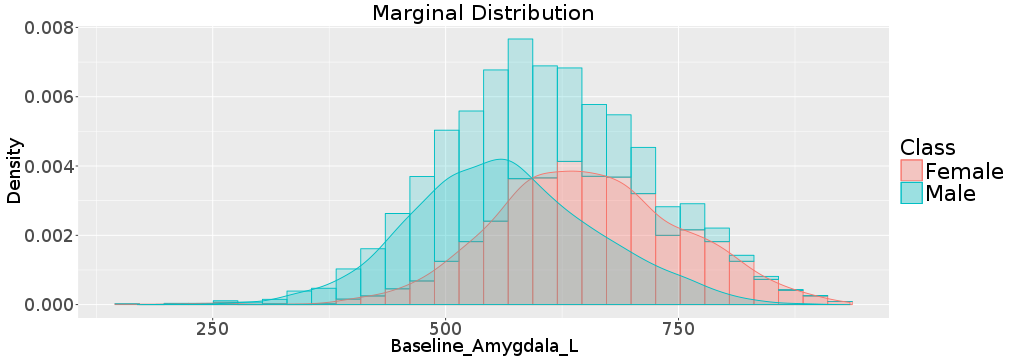
\includegraphics[width=\textwidth,valign=t]{Figures/Spect_Gender/Baseline_Amygdala_L_Marginal.png}
		\subcaption{}
		\label{fig:FigSpecMarginal}
	\end{subfigure}
	%\vspace{-3\baselineskip}
	\caption{Marginal distribution of the baseline image left amygdala feature with (a) raw data and (b) data stratified by gender. Note that there is visible separation between classes.}
	\label{fig:FigSpectMarginalCaption}
\end{figure}

We next used MX to explore a previously unanalyzed SPECT dataset composed of 4,283 individuals. For each individual the data set contained two images, a baseline image which was acquired while the patient was at rest and a concentration image which was acquired while the patient underwent a concentration task. Both images were converted to a Matrix Explorer friendly format by mapping the resultant SPECT image data onto a standard brain atlas, segmenting the brain into 128 voxels, and computing the average intensity within that voxel. As a result, each patient row in the corresponding dataset has 256 features along with associated patient information. For the purposes of this work, we specifically explored the relationship between the feature columns and the associated patient gender. 

A characteristic feature marginal, showing the distribution of average intensity in the left amygdala in the baseline image, is shown in Figure~\ref{fig:FigSpecNoClassMarginal}. The resultant marginal after conditioning on gender is shown in Figure~\ref{fig:FigSpecMarginal}. Note that some clear separation is visible between the marginals of the two classes. This trend is visible in nearly all the marginals, suggesting that there is a difference in the SPECT images between genders.

We can also gain useful information by examining the robust distances of each patient and by examining how these distances relate to their gender. The corresponding figure is shown in Figure~\ref{fig:FigSpecOutlierPlot}. The robust distances for female patients tended to be greater than those for male patients, corroborating the results seen in the feature marginals.

\begin{figure}[t]
	\centering
	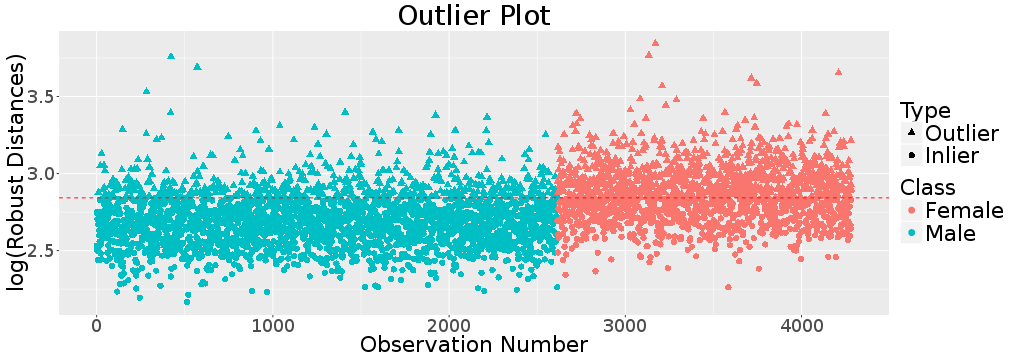
\includegraphics[width=0.48\textwidth,valign=t]{Figures/Spect_Gender/OutlierPlot.png}
	\caption{Plot of robust distances for all individuals colored based on gender. Note that female patients tend to have a greater distance.}
	\label{fig:FigSpecOutlierPlot}
\end{figure}

\section{Conclusion}
\label{sec:conc}

We have created MX, a web application driven by the R Shiny package, which allows for basic data exploration and visualization of small to medium sized datasets. Within MX, we have included the tools whose usage we believe to be best practice whenever exploring a new dataset. We have validated the functionality of MX by demonstrating its capability to characterize the iris flower dataset and determine the presence of three different classes. We have then used MX to explore a previously uncharacterized dataset, a collection of SPECT images from over 4000 patients, and show an interesting association between SPECT image voxel intensities and gender. This latter finding merits further investigation.

Although the implemented algorithms may seem simplistic to those with a statistical background, they are highly relevant to MXs target user base: scientists with minimal knowledge of statistical techniques who would otherwise be unable to properly analyze their data. As such, MX helps resolves a very important issue, and is the a small step in the process of enabling anyone to use statistical tools to examine their data.

\section{Acknowledgments}
\label{sec:ack}
We would like the thank Daniel Amen for providing the SPECT data.

\bibliographystyle{Chicago}
\bibliography{BibliographyMX}
\end{document}
